
\section{Introduction to Rotation\footnote{
1990-93 Dept. of Physics and Astronomy, Dickinson College. Supported by FIPSE
(U.S. Dept. of Ed.) and NSF. Portions of this material may have been modified
locally and may not have been classroom tested at Dickinson College.
}}

\makelabheader %(Space for student name, etc., defined in master.tex or labmanual_formatting_commands.tex)

\textbf{Objectives} 

To understand the definitions of angular velocity and angular acceleration and
the kinematic equations for rotational motion on the basis of observations.
We will discover the relationship between linear velocity and angular velocity
and between linear acceleration and angular acceleration.

\textbf{Apparatus}

\begin{itemize}
\item A rotator consisting of an axle, a metal disk, and a fixture to hold the disk. 
\item A stopwatch. 
\item A meter stick, drawing compass, flexible ruler, protractor, and some string.
\end{itemize}
\textbf{Overview }

Earlier in the course, we studied centripetal force and acceleration, which
characterize circular motion. In general, however, we have focused on studying
motion along a straight line as well as the motion of projectiles. We have defined
several measurable quantities to help us describe linear and parabolic motion,
including position, velocity, acceleration, force, and mass. In the real world,
many objects undergo circular motion and/or rotate while they move. The electron
orbiting a proton in a hydrogen atom, an ice skater spinning, and a hammer that
tumbles about while its center of mass moves along a parabolic path are just
three of many rotating objects. 

Since many objects undergo rotational motion it is useful to be able to describe
their motions mathematically. The study of rotational motion is also very useful
in obtaining a deeper understanding of the nature of linear and parabolic motion.

We are going to try to define several new quantities and relationships to help
us describe the rotational motion of rigid objects, i.e., objects that do not
change shape. These quantities will include angular velocity, angular acceleration,
rotational inertia and torque. We will then use these new concepts to develop
an extension of Newton's second law to describe rotational motion for masses
more or less concentrated at a single point in space (e.g., the electron in
the hydrogen atom) and for extended objects (like the tumbling hammer).

\textbf{Rigid \textit{vs.}~Non-rigid Objects} 

We will begin our study of rotational motion with a consideration of some characteristics
of the rotation of rigid objects about a fixed axis of rotation. The motions
of objects, such as clouds, that change size and shape as time passes are hard
to analyze mathematically. In this unit we will focus primarily on the study
of the rotation of particles and rigid objects around an axis that is not moving.
A rigid object is defined as an object that can move along a line or can rotate
without the relative distances between its parts changing. 

Shown in the figure below are examples of a non-rigid object in the form of
a cloud that can change shape and of a rigid object in the form of an empty
coffee cup that does not change shape.

\vspace{0.3cm}
{\par\centering 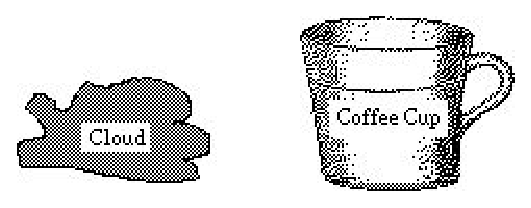
\includegraphics{rotation/rotation_fig1.eps} \par}
\vspace{0.3cm}

A hammer tossed end over end and an empty coffee cup are examples of rigid objects.
A ball of clay that deforms permanently in a collision and a cloud that grows
are examples of non-rigid objects. 
\vspace{0.3cm}

\textbf{A Puzzler} 

Use your imagination to solve the rotational puzzler outlined below. It's one
that might stump someone who hasn't taken physics.

\textbf{Activity 1: Horses of a Different Speed }

You are on a white horse, riding off at sunset with your beau on a chestnut
mare riding at your side. Your horse has a speed of 4.0 m/s and your beau's
horse has a speed of 3.5 m/s, yet he/she constantly remains at your side. Where
are your horses? Make a sketch to explain your answer.

\vspace{0.3cm}
{\par\raggedright 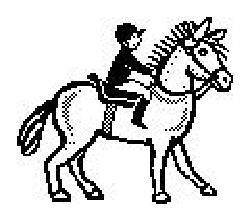
\includegraphics{rotation/rotation_fig3.eps} \par}
\vspace{0.3cm}

\textbf{Review of the Geometry of Circles }

Remember way back before you came to college when you studied equations for
the circumference and the area of a circle? Let's review those equations now,
since you'll need them a lot from here on in.

\textbf{Activity 2: Circular Geometry} 

(a) What is the equation for the circumference, $C$, of a circle of radius $r$?
What are the units of $C$?

\vspace{0.3cm}
{\par\raggedright 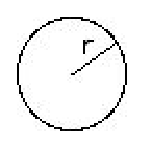
\includegraphics{rotation/rotation_fig4.eps} \par}
\vspace{0.3cm}

(b) What is the equation for the area, $A$, of a circle of radius r? What are
the units of $A$?
\vspace{10mm}

(c) If someone told you that the area of a circle was $A = r$, how could you refute
them immediately? What's wrong with the idea of area being proportional to $r$?
\vspace{20mm}

\textbf{Distance from an Axis of Rotation and Speed }

Let's begin our study by examining the rotation of objects about a common axis
that is fixed. What happens to the speeds of different parts of a rigid object
that rotates about a common axis? How does the speed of the object depend on
its distance from an axis? You should be able to answer this question by observing
the rotational speed of the rotator at each experimental station.

\vspace{0.3cm}
{\par\centering 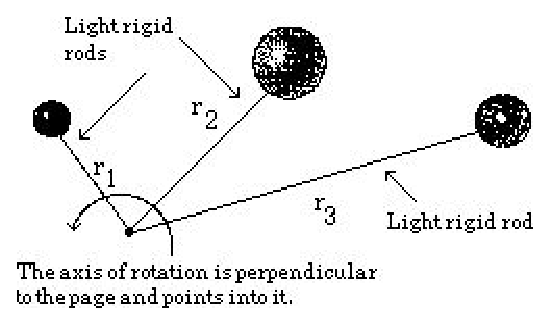
\includegraphics[scale=0.8]{rotation/rotation_fig5.eps} \par}
\vspace{0.3cm}

Place the disk in the fixture and slowly rotate it a constant speed. The figure
below shows the rotator and the definition of angular displacement.

\vspace{0.3cm}
{\par\centering 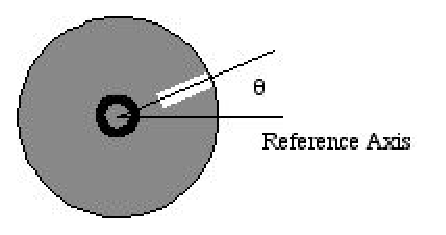
\includegraphics[scale=0.8]{rotation/rotation_fig6.eps} \par}
\vspace{0.3cm}

\textbf{Activity 3: Spinning the Rotator: Speed \textit{vs.}~Radius} 

(a) Measure how long it takes the white marker to sweep through a known angle.
Record the time and the angle in the space below.
\answerspace{10mm}

(b) Calculate the distance of the paths traced out by the outer edge of the white marker and the inner edge as it rotated through the angle you just recorded.
(Note: What do you need to measure to perform this calculation?) Record your
data below.
\answerspace{20mm}

(c) Calculate the average speed of the outer edge of the white marker and the
average speed of the inner edge of the marker. How do they compare?
\answerspace{20mm}

(d) Do the speeds seem to be related in any way to the distances of inner and
outer edges of the white marker from the axis of rotation? If so, describe the
relationship mathematically.
\answerspace{18mm}

\pagebreak[2]
(e) As the disk rotates, does the distance from the axis of rotation to the outer edge of the white marker change?
\answerspace{10mm}

(f) As the disk rotates, does the distance from the axis of rotation to the inner edge of the white marker change?
\vspace{10mm}

(g) At any given time during your rotation, is the angle between the reference
axis and the inner edge of the white marker the same as the angle between the
axis and the outer edge of the white marker, or do the angles differ?
\vspace{10mm}

(h)At any given time during the rotation, is the rate of change of the angle
between the reference axis and the inner edge of the white marker the same as
the rate of change of the angle between the axis and the outer edge, or do the
rates differ?
\vspace{10mm}

(i) What happens to the linear velocity, \textbf{v}, of the outer edge of the
marker as it rotates at a constant rate? Hint: What happens to the magnitude
of the velocity, i.e., its speed? What happens to its direction?
\vspace{20mm}

(j) Is the outer edge of the white marker accelerating? Why or why not?
\vspace{20mm}

\textbf{Radians, Radii, and Arc Lengths} 

An understanding of the relationship between angles in radians, angles in degrees, and arc lengths is critical in the study of rotational motion. There are two
common units used to measure angles: degrees and radians.

\begin{enumerate}
\item A degree is defined as 1/360th of a rotation in a complete circle.
\item A radian is defined as the angle for which the arc along the circle is equal to its radius as shown in the figure below.
\end{enumerate}
\vspace{0.3cm}
{\par\centering 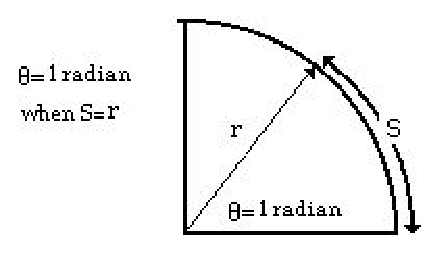
\includegraphics{rotation/rotation_fig7.eps} \par}
\vspace{0.3cm}

In the next series of activities you will be relating angles, arc lengths, and
radii for a circle.

\pagebreak[2]
\textbf{Activity 4: Relating Arcs, Radii, and Angles} 

(a) Let's warm up with a review of some very basic mathematics. What should
the constant of proportionality be between the circumference of a circle and
its radius? Write the appropriate equation.
\answerspace{10mm}

(b) Approximately how many degrees are in one radian? Let's do this experimentally.
Using the compass draw a circle and measure its radius. Then, use the flexible
ruler to trace out a length of arc, s, that has the same length as the radius.
Next measure the angle in degrees that is subtended by the arc.
\answerspace{40mm}

(c) Theoretically, how many degrees are in one radian? Please calculate your
result to three significant figures. Using the equation for the circumference
of a circle as a function of its radius and the constant $\pi=3.1415927$..., 
figure
out a general equation to find degrees from radians. \textbf{Hint:} How many
times does a radius fit onto the circumference of a circle? How many degrees
fit in the circumference of a circle?
\answerspace{20mm}

(d) If an object moves 30 degrees on the circumference of a circle of radius
1.5 m, what is the length of its path?
\answerspace{20mm}

(e) If an object moves 0.42 radians on the circumference of a circle of radius
1.5 m, what is the length of its path?
\answerspace{20mm}

(f) Remembering the relationship between the speed of the outer edge of the
rotator and the distance, $r$, 
from the rotator's axis the outer edge, what equations
would you use to define the magnitude of the average ``angular''
velocity, \( \langle\omega \rangle \)? \textbf{Hint:} In words, 
\( \langle\omega \rangle \) is defined
as the amount of angle swept out by the object per unit time. Note that the
answer is not simply \( \theta/t  \)!

\vspace{0.3cm}
{\par\raggedright 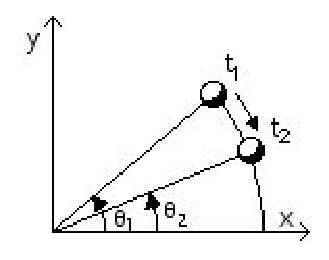
\includegraphics{rotation/rotation_fig8.eps} \par}
\vspace{0.3cm}

(g) How many radians are there in a full circle consisting of 360 degrees?
\vspace{10mm}

(h) When an object moves in a complete circle in a fixed amount of time, what
quantity (other than time) remains unchanged for circles of several different
radii? 
\vspace{10mm}

\textbf{Relating Linear and Angular Quantities} 

It's very useful to know the relationship between the variables 
$s$, $v$, and $a$,
which describe linear motion and the corresponding variables \( \theta  \),
\( \omega  \), and \( \alpha  \), which describe rotational motion. You now
know enough to define these relationships.

\textbf{Activity 5: Linear and Angular Variables }

(a) Using the definition of the radian, what is the general relationship between
a length of arc, $s$, on a circle and the variables 
$r$ and \( \theta  \) in radians. 
\vspace{10mm}

(b) Assume that an object is moving in a circle of constant radius, $r$. Using the relationship you found in part (a) above, take the derivative of s with respect to time to find the velocity of the object. Show that the magnitude of the linear velocity, $v$, is related to the magnitude of the angular velocity,
\( \omega  \), by the equation \(v =  \omega r \).
\vspace{20mm}

(c) Assume that an object is accelerating in a circle of constant radius, $r$.
Using the relationship you found in part (b) above, take the derivative of $v$ with respect to time to find the tangential acceleration of the object. Show that the linear acceleration, \( a_{t} \), tangent to the circle is related to the angular acceleration, \( \alpha  \), by the equation \( a_{t}  =  \alpha  r\).
\vspace{20mm}

\textbf{The Rotational Kinematic Equations for Constant \( \alpha  \) }

The set of definitions of angular variables are the basis of the physicist's
description of rotational motion. We can use them to derive a set of kinematic
equations for rotational motion with constant angular acceleration that are
similar to the equations for linear motion. 

\newpage
\textbf{Activity 6: The Rotational Kinematic Equations }

The figure below shows a massless string wound around a spool of radius $r$.
The mass falls with a constant acceleration, $a$. Refer to this figure and the 
results of Activity 5 to answer the following questions. NOTE: The distance 
$y$ that the mass falls is equal to the arc length $s$ moved by a point on the 
edge of the spool.

\vspace{0.3cm}
{\par\centering 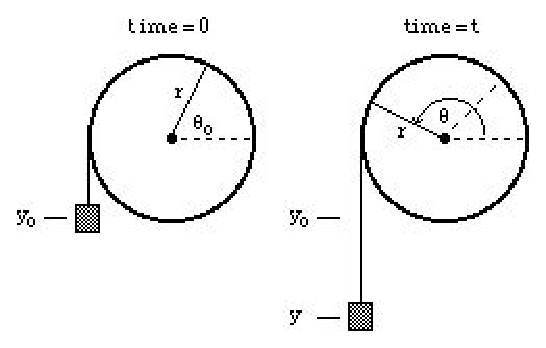
\includegraphics{rotation/rotation_fig9.eps} \par}
\vspace{0.3cm}

(a) What is the equation for \( \theta  \) in terms of $y$ and $r$?
\vspace{10mm}

(b) What is the equation for \( \omega  \) in terms of $v$ and $r$?
\vspace{10mm}

(c) What is the equation for \( \alpha  \) in terms of $a$ and $r$?
\vspace{10mm}

(d) Consider the falling mass in the figure above. Note that the positive 
y-axis is pointing down. Using the 
relationships between the linear and angular variables in parts (a), (b), and 
(c), derive the rotational kinematic equation for constant acceleration for 
each linear kinematic equation listed below. \textbf{Warning:} Don't just write
the analogous equations! Show the substitutions needed to derive the equations
on the right from those on the left.

\begin{enumerate}
\item \( v=v_{0}+at\qquad \qquad \qquad \omega = \)\vspace{20mm}

\item \( y=y_{0}+v_{0}t+\frac{1}{2}at^{2}\qquad \qquad \theta = \)\vspace{20mm}

\item \( v^{2}=v_{0}^{2}+2ay\qquad \qquad \qquad \omega ^{2}= \)
\end{enumerate}
